% !TEX root = thesis.tex

\newpage
\chapter{Numerical approximations}
In order to solve conservation laws of the form \eqref{eq:conslaw} we usually assume smooth initial conditions $\rho(x,0)$. We are naturally interested in the difficulties caused by discontinuities in the solution. Straight-forward numerical methods like the finite difference approximation usually have difficulties near the discontinuity. Consider for instance the scalar (linear) advection equation 
\begin{eqnarray}
\label{eq:advection}
&u_t+Au_x=0, \hspace{0,5cm} -\infty<x<\infty, t\geq 0 \nonumber \\
&u(x,0)=\begin{cases} 1 \hspace{0,5cm} x<0\\ 0  \hspace{0,5cm} x>0 \end{cases}  
\end{eqnarray}
Obviously the analytical solution obtained by the method of characteristics is given by a travelling show wave $u(x,t)=u_0(x-At)$ with wave speed $A$.
\textcolor{red}{ADD Lax Equivalence Theorem?? }
Unfortunately the finite difference approach is inconsistent, as the finite difference approximation to $u_x$ at the discontinuity $x=0$ will not approach 0, e.g.
\begin{equation*}
	u_x\sim\frac{u_0(At+h)-u_0(At-h)}{2h}=\frac{0-1}{2h}\rightarrow-\infty, \text{ as } h\rightarrow 0
\end{equation*}
In particular, the \textit{local truncation error} 
\begin{equation}
L_k(0,t):=\frac{1}{k}\left[u(0,t+k)-u(0,t)\right]-a\frac{u_0(At+h)-u_0(At-h)}{2h}
\end{equation}
for the finite difference scheme does not vanish for $h,k\rightarrow 0$ (see also \citep{LeVeque.1992}). A numerical method of \textbf{order p} fulfills that $L_k(x,t)=\mathcal{o}(k^p)$. This means that the finite difference scheme for discontinuous data does neither provide local nor global convergence towards the analytical solution. \newline
\newline
For linear systems of the form \eqref{eq:advection} a wide variety of convergent numerical methods using adjusted finite difference schemes are given. Some possibilites are stated in Table \ref{schemes}. 
\begin{table}[h]
\renewcommand{\arraystretch}{2}%
\begin{tabular}{|l|l|c|}
\hline  
Name & Difference equation & Order  \\ \hline
Lax-Friedrich & $\begin{array}{lcl}
u(x,t+k)&=&\frac{1}{2}\left(u(x+h,t)+u(x-h,t)\right) \\
&-&\frac{k}{2h}A(u(x+h,t)-u(x-h,t))
\end{array}$ & 1\\
Upwind $(A>0)$& $\begin{array}{lcl}u(x,t+k)&=&u(x,t)-\frac{k}{2h}A(u(x,t)-u(x-h,t))\end{array}$ & 1 \\
Lax-Wendroff & $\begin{array}{lcl}
u(x,t+k)&=&u(x,t)-\frac{k}{2h}A(u(x+h,t)-u(x-h,t)) \\
&+&\frac{k^2}{2h^2}A^2\left(u(x+h,t)-2u(x,t)+u(x-h,t)\right)
\end{array}$ & 2 \\
Beam-Warming & $\begin{array}{lcl}
u(x,t+k)&=&u(x,t)-\frac{k}{2h}A(3u(xh,t)-4u(x-h,t) \\
&+&u(x-2h,t))+\frac{k^2}{2h^2}A^2((u(xh,t)\\&-&2u(x-h,t)+u(x-2h,t))
\end{array}$ & 2 \\
\hline
\end{tabular}
\caption{\label{schemes}Finite difference schemes for the linear advection problem \eqref{eq:advection}.}
\end{table}
First order method (Upwind, Lax-Friedrich) typically produce a flattened solutions compared to the original solutions, whereas second order methods (Lax-Wendroff and Beam-Warming) give oscillations. These phenomena are displayed in Figure \ref{fig:schemes}. 
\begin{figure}[h]
\center
\includegraphics[scale=0.4]{numeric_schemes}
\caption{\label{fig:schemes} Numerical and exact solution of conservation law \eqref{eq:advection}} at $t=0.5$ and step size $h=0.0025$ using the following methods (top left to bottom right) (a) Lax-Friedrich, (b) Upwind, (c) Lax-Wendroff, (d) Beam-Warming
\end{figure}
\section{The Godunov scheme for nonlinear conservation laws}
Finite difference schemes as discussed in the introductive part of this chapter provide \textit{smooth} solutions, even if the initial datum of the conservation law contains discontinuities and jumps. Even to nonlinear problems these PDEs can often be linearized and therefore results from the linear FD methods applied in order to obtain convergence results for nonlinear problems \citep{Strang}. There are several limitations to this approach: \newline Firstly it is not guaranteed that the obtained numerical solution really converges towards the analytical discontinuous solution (see e.g. Burger's equation). Secondly the modelling of travelling waves, in particular the evolution of traffic jams and shocks often emerge from initial discontinuities discontinuities. Thus a different approach has to be persued. \newline
\subsection{Theory of conservative numerical schemes}
Let us consider the x-t-plane as the operating space. We can discretize this space by choosing a mesh with step size $h:=\Delta x$ and time step $k:=\Delta t$, $\frac{h}{k}=C>0$ fixed. In particular the mesh points are given by
\begin{eqnarray*}
	x_j&=&jh, \hspace{1cm} j=\dots,-1,0,1,\dots \\
	t_n&=&nk, \hspace{1cm} n=0,1,\dots
\end{eqnarray*}
We also define the midpoints in space 
\begin{equation*}
	x_{j\pm\frac{1}{2}}:=x_j\pm\frac{h}{2}
\end{equation*}
We can now define the \textbf{cell averages} of the density $\rho(x,t)$ on the mesh as
\begin{equation}
u_j^n:=\int_{x_{j-\frac{1}{2}}}^{x_{j+\frac{1}{2}}}\rho(x,t_n)dx
\end{equation}
The idea of the \textbf{Godunov scheme} is to approximate the solution $\rho(x,t_n)$ to conservation law \eqref{eq:integral_form} by a piecewise constant function 
\begin{equation}
u^n(x,t_n)=u_j^n \hspace{1cm} \text{if} \ x_{j-\frac{1}{2}}\leq x < x_{j+\frac{1}{2}}
\end{equation}
 and by solving the Riemann problems caused by the space discretization on the time interval $[t_n,t_{n+1}]$. 
Following from the integral form of conservation law \eqref{eq:integral_form}, namely
\begin{eqnarray}
\int_{x_{j-\frac{1}{2}}}^{x_{j+\frac{1}{2}}}\rho(x,t_{n+1})dx &=& \int_{x_{j-\frac{1}{2}}}^{x_{j+\frac{1}{2}}}\rho(x,t_{n})dx \\
&&-\left[\int_{t_{n}}^{t_{n+1}}f(\rho(x_{j+\frac{1}{2}},t))dt-\int_{t_{n}}^{t_{n+1}}f(\rho(x_{j-\frac{1}{2}},t))dt\right] \nonumber
\end{eqnarray}
we obtain \begin{equation}
\label{eq:conservative}
u_j^{n+1}=u_j^n-\frac{1}{h}\left[\int_{t_{n}}^{t_{n+1}}f(\rho(x_{j+\frac{1}{2}},t))dt-\int_{t_{n}}^{t_{n+1}}f(\rho(x_{j-\frac{1}{2}},t))dt\right]
\end{equation}
with the \textbf{numerical flux function} 
\begin{equation}
\label{eq:num_flux}
F(u_j^n,u_{j+1}^n)\sim \frac{1}{k}\int_{t_n}^{t_{n+1}}f(\rho(x_{j+\frac{1}{2}},t)dt
\end{equation}
which plays the role of the average flux through $x_{j+\frac{1}{2}}$ over the time interval $[t_n,t_{n+1}]$. Numerical methods of the form \eqref{eq:conservative} are called \textit{in conservative form} as they still fulfill the conservation law. 
\newline
\newline
We also note that in practise equation \ref{eq:num_flux} simplifies since $u_j^n$ at point $x_{j+\frac{1}{2}}$ is constant along the line $[t_n,t_{n+1}]$ (also see picture \textcolor{red}{ADD picture like LeVeque p.139}.  Therefore the numerical flux at point $x_{j+\frac{1}{2}}$ only depends on the neighboring densities $u_j^n$ and $u_{j+1}^n$. Denoting this value by $u^*(u_j^n,u_{j+1}^n$ the numerical flux reduces to
\begin{equation}
F(u_j^n,u_{j+1}^n)=f(u^*(u_j^n,u_{j+1}^n))
\end{equation}
Obviously the scheme is consistent, since $F(u_j^n,u_{j}^n)=f(u_j^n))$. \newline
We mentioned earlier that $u_j^n$ at $x_{j+\frac{1}{2}}$ is constant along the line $[t_n,t_{n+1}]$. This only holds if the cells are "small enough" such that two shocks resulting from neighboring Riemann problems do not interact between two time steps. As the wave speed is bounded by the eigenvalue of $f'(u)$ we require that \begin{equation}
c_C:=\frac{k}{h}|\sup(f'(u))|\leq 1
\end{equation} 
$c_C$ is also called the Courant-number and serves as the one-dimensional CFL-condition \citep{Courant.1928}.
\newline
\newline
The \textbf{Godunov method} now consists of seperately solving every Riemann problem between every two neighboring cells. Let $u_j$ and $u_{j+1}$ be the densities on two neighboring cells. Then the flux $f(u^*(u_j,u_{j+1})$ is given by
\begin{equation}
\label{eq:numerical_flux}
f(u^*(u_j,u_{j+1}))=\begin{cases} \min \left[f(u_j),f(u_{j+1})\right] \hspace{1cm}\text{if} \ u_l\leq u_r \\
%f(\sigma)\hspace{1cm}\text{if} \ u_r\leq\sigma\leq u_l \\
%f(u_r) \hspace{1cm}\text{if} \ \sigma\leq u_r \leq u_l \\
%f(u_l) \hspace{1cm}\text{if} \  u_r\leq u_l\leq\sigma
\max \left[f(u_j),f(u_{j+1})\right] \hspace{1cm}\text{if} \ u_l\geq u_r
\end{cases}
\end{equation}
This form of the resulting flux function is valid for any general scalar conservation laws, even for nonconvex fluxes.
In the convex case we can distinguish 4 cases for the numerical flux \eqref{eq:numerical_flux}, see Figure \ref{fig:solution_types}:
\begin{enumerate}
\item $f'(u_j),f'(u_{j+1})\geq 0$: Here the solution consists of a rarefaction wave with $u^*(u_l,u_r)=u_j$.
\item $f'(u_j),f'(u_{j+1})\leq 0$: The solution consists of a rarefaction wave with $u^*(u_l,u_r)=u_{j+1}$.
\item $f'(u_{j+1})<0\leq f'(u_j)$: Then there is a shock through $x_{j+\frac{1}{2}}$ and \begin{equation*}
u^*(u_j,u_{j+1})=\begin{cases} u_j &: s\geq 0 \\
u_{j+1} &:s<0\end{cases}
\end{equation*}
with the shock speed \begin{equation*}
s=\frac{f(u_{j+1})-f(u_j)}{u_{j+1}-u_j}
\end{equation*}
\item $f'(u_{j+1})>0\geq f'(u_j)$: In this case we have the so-called transonic rarefaction wave and $u^*(u_j,u_{j+1})=\sigma$, with $u=\sigma$ the unique point at which $f'(u)=0$ (cf. \eqref{eq:max_flux}).
\end{enumerate}
\begin{figure}[h]
\center
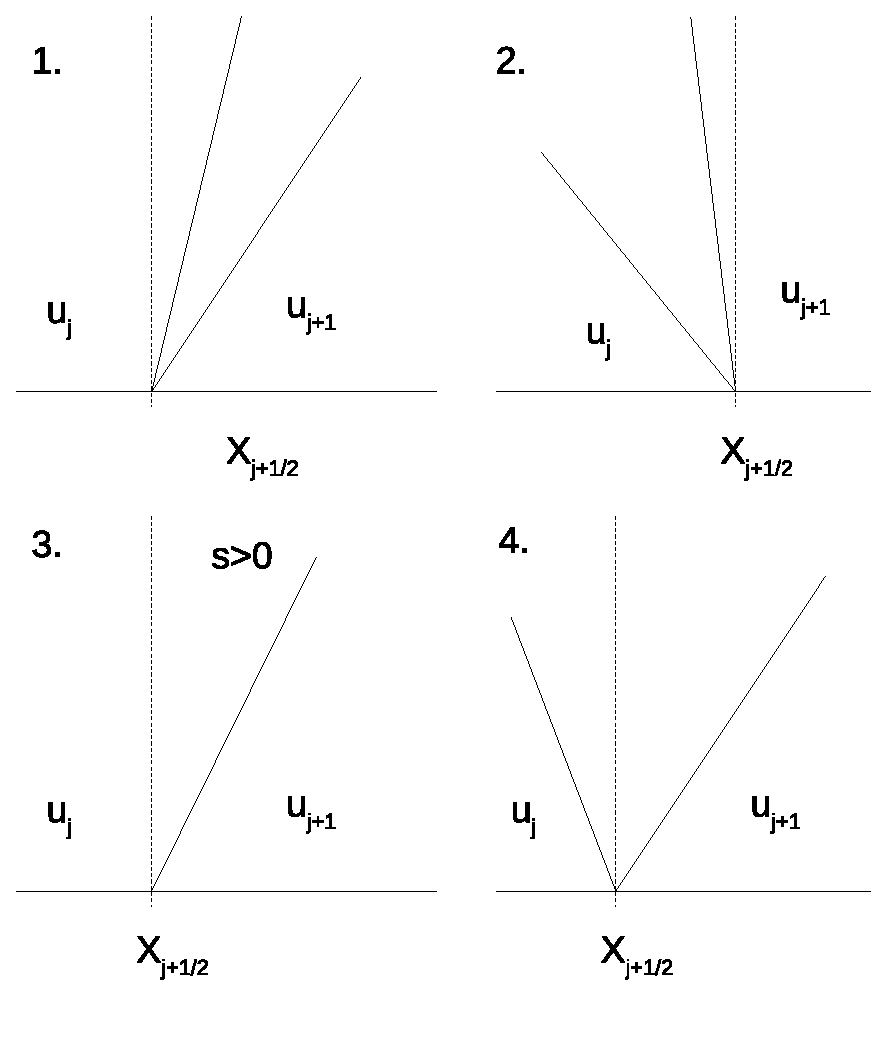
\includegraphics[scale=0.6]{figures/solution_types}
\caption{\label{fig:solution_types} Different types of solutions for the Riemann problem dependent on densities $u_j^n$ and $u_{j+1}^n$.}
\end{figure} \newline
\newline
In the following we want to apply the Godunov scheme on the buffer model defined in section \ref{buffer_model}.
\subsection{The Godunov scheme for the buffer model}
Let us consider an arbitrary connected road network $(\mathcal{N},\mathcal{E})$ with $n_R$ roads and $n_J$ junctions. On every road $e_i=[a_i,b_i]$ we apply the discretization $x_{i,j}=a_{i,jh}, j=0,...,D_i, x_{i,D_ih}=b_i$, with $D_i=\frac{b_i-a_i}{h}-1$ the number of cells on road $e_i$. Let us then denote $u_{i,j}^n$ the density on the j-th cell of road $e_i$ at time $t=nk$.\newline
\newline
We can now define on all \textit{inner cells} of every road $e_i$ the Godunov scheme 
\begin{subequations}
\label{eq:Godunov}
\begin{equation}
u_{i,j}^{n+1}=u_{i,j}^n-\frac{k}{h}\left[f(u^*(u_{i,j}^n,u_{i,j+1}^n))-f(u^*(u_{i,j-1}^n,u_{i,j}^n))\right],\hspace{1cm} e_i\in\mathcal{E}, j=1,\dots,D_i-1
\end{equation}  
We incorporate the \textit{externally inflowing densities} $q_i(t), e_i\in\mathcal{E}^{in}$ by introducing a ghost cell at the beginning of each road $e_i$. Then we define 
\begin{equation}
u_{i,0}^{n+1}=u_{i,0}^n-\frac{k}{h}\left[f(u^*(u_{i,0}^n,u_{i,1}^n)-f(u^*(v_{i,1}^n,u_{i,0}^n)) \right], \hspace{1cm} i\in\mathcal{E}^{in}
\end{equation} 
with the inflowing density $v_{i,1}^n:=\int_{t_n}^{t_{n+1}}\rho_{in,i}(t)dt$. \newline
The outfluxes leaving the network can be treated analogously. \newline
\newline
For junctions we recall equations \eqref{eq:sbj} for the junction fluxes in the single buffer model. Accordingly, we define for roads coming into junction $J$
\begin{equation}
u_{i,D_i}^{n+1}=u_{i,D_i}^n-\frac{k}{h}\left[\bar{f}_i-f(u^*(u_{i,D_i-1}^n,u_{i,D_i}^n)) \right], \hspace{1cm} i\in\delta^{in}(J)
\end{equation}
For outgoing roads of junction $J$ we analogously define the scheme
\begin{equation}
u_{i,0}^{n+1}=u_{i,0}^n-\frac{k}{h}\left[f(u^*(u_{i,0}^n,u_{i,1}^n))-\hat{f}_i \right], \hspace{1cm} i\in\delta^{out}(J)
\end{equation}
\end{subequations}
\underline{\textbf{Remarks:}}\begin{itemize}
\item For the computation of the buffer, which is needed for the junction fluxes, we use a simple difference quotient to approximate $\dot{q}$,
\begin{equation}
	q_j^{n+1}=q_j^n+k\left[\sum_{i\in\delta^{in}(J)}\bar{\Theta}_{i,j}\bar{f_i}-\bar{f_j}\right], \hspace{1cm}J\in\mathcal{N},j\in\delta^{out}(J)
\end{equation}
\item For convenience we condense equations \eqref{eq:Godunov}a-d on road $e_i$ to the condensed Godunov scheme 
\begin{equation}
u_i^{n+1}=G(u_i^n)
\end{equation}
\end{itemize} 
\section{Examples}
